% $Id: template.tex 11 2007-04-03 22:25:53Z jpeltier $
\newcommand{\todo}[1]{{\bf \{TODO: {#1}\}}}
\newcommand{\projectname}{Story Explorer}

\documentclass{vgtc}                          % final (conference style)
%\documentclass[review]{vgtc}                 % review
%\documentclass[widereview]{vgtc}             % wide-spaced review
%\documentclass[preprint]{vgtc}               % preprint
%\documentclass[electronic]{vgtc}             % electronic version

%% Uncomment one of the lines above depending on where your paper is
%% in the conference process. ``review'' and ``widereview'' are for review
%% submission, ``preprint'' is for pre-publication, and the final version
%% doesn't use a specific qualifier. Further, ``electronic'' includes
%% hyperreferences for more convenient online viewing.

%% Please use one of the ``review'' options in combination with the
%% assigned online id (see below) ONLY if your paper uses a double blind
%% review process. Some conferences, like IEEE Vis and InfoVis, have NOT
%% in the past.

%% Figures should be in CMYK or Grey scale format, otherwise, colour 
%% shifting may occur during the printing process.

%% These three lines bring in essential packages: ``mathptmx'' for Type 1 
%% typefaces, ``graphicx'' for inclusion of EPS figures. and ``times''
%% for proper handling of the times font family.

\usepackage{mathptmx}
\usepackage{graphicx}
\usepackage{times}

%% We encourage the use of mathptmx for consistent usage of times font
%% throughout the proceedings. However, if you encounter conflicts
%% with other math-related packages, you may want to disable it.

%% If you are submitting a paper to a conference for review with a double
%% blind reviewing process, please replace the value ``0'' below with your
%% OnlineID. Otherwise, you may safely leave it at ``0''.
\onlineid{0}

%% declare the category of your paper, only shown in review mode
\vgtccategory{Research}

%% allow for this line if you want the electronic option to work properly
\vgtcinsertpkg

%% In preprint mode you may define your own headline.
%\preprinttext{To appear in an IEEE VGTC sponsored conference.}

%% Paper title.

\title{\projectname: A Visual Analysis Tool for News Data}

%% This is how authors are specified in the conference style

%% Author and Affiliation (single author).
%%\author{Roy G. Biv\thanks{e-mail: roy.g.biv@aol.com}}
%%\affiliation{\scriptsize Allied Widgets Research}

%% Author and Affiliation (multiple authors with single affiliations).
%%\author{Roy G. Biv\thanks{e-mail: roy.g.biv@aol.com} %
%%\and Ed Grimley\thanks{e-mail:ed.grimley@aol.com} %
%%\and Martha Stewart\thanks{e-mail:martha.stewart@marthastewart.com}}
%%\affiliation{\scriptsize Martha Stewart Enterprises \\ Microsoft Research}

%% Author and Affiliation (multiple authors with multiple affiliations)
\author{Roy G. Biv\thanks{e-mail: roy.g.biv@aol.com}\\ %
        \scriptsize Starbucks Research %
\and Ed Grimley\thanks{e-mail:ed.grimley@aol.com}\\ %
     \scriptsize Grimley Widgets, Inc. %
\and Martha Stewart\thanks{e-mail:martha.stewart@marthastewart.com}\\ %
     \parbox{1.4in}{\scriptsize \centering Martha Stewart Enterprises \\ Microsoft Research}}

%% A teaser figure can be included as follows, but is not recommended since
%% the space is now taken up by a full width abstract.
%\teaser{
%  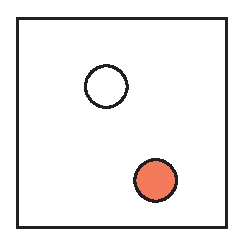
\includegraphics[width=1.5in]{sample.eps}
%  \caption{Lookit! Lookit!}
%}

%% Abstract section.
\abstract{\todo{Add the abstract after complete the summary}
} % end of abstract

%% ACM Computing Classification System (CCS). 
%% See <http://www.acm.org/class/1998/> for details.
%% The ``\CCScat'' command takes four arguments.

\CCScatlist{ 
  \CCScat{K.6.1}{Management of Computing and Information Systems}%
{Project and People Management}{Life Cycle};
  \CCScat{K.7.m}{The Computing Profession}{Miscellaneous}{Ethics}
}

%% Copyright space is enabled by default as required by guidelines.
%% It is disabled by the 'review' option or via the following command:
% \nocopyrightspace

%%%%%%%%%%%%%%%%%%%%%%%%%%%%%%%%%%%%%%%%%%%%%%%%%%%%%%%%%%%%%%%%
%%%%%%%%%%%%%%%%%%%%%% START OF THE PAPER %%%%%%%%%%%%%%%%%%%%%%
%%%%%%%%%%%%%%%%%%%%%%%%%%%%%%%%%%%%%%%%%%%%%%%%%%%%%%%%%%%%%%%%%

\begin{document}

%% The ``\maketitle'' command must be the first command after the
%% ``\begin{document}'' command. It prepares and prints the title block.

%% the only exception to this rule is the \firstsection command
\firstsection{Introduction}

\maketitle

Exploring heterogeneous news data from different sources can be complicated and error pruning if not well dealt with hidden relationship between entities or possible data conflicts between materials. 
In the MC1 of VAST Challenge 2014, to extract relationship between POK and GAStech we need to extract important people from different sources of file, e.g. employee resume, email, research report, and a huge volume of news with conflicts. 
In our design of the analysis tool \projectname\ we integrate different kinds of source files into a timeline-based view, providing a quick overview for user to choose important file to focus for efficiency. 
\par
In this poster, we will first introduce our design consideration of visual analysis tools for heterogeneous data and then introduce how we use these tools to analyze MC1 data to solve these problems.
%% \section{Introduction} 

%eg.\cite{kitware2003,Max:1995:OMF}

\section{Design Challenges}
Data provided in MC1 mainly includes 845 news articles, 35 resumes, employee records, email headers and some other report on both POK and Kronos. As the data volume is large, we need to provide an efficient overview to put important data together. Challenges we face in our design of \projectname\ focus are listed below:
\paragraph{Data correlation and data conflicts}
In MC1, data are overlapping and thus there exists correlation and conflicts. For example, both resume and employee records present GAStech employee information, and report on POK and Kronos cover some information in news articles. And thus we have challenges to present data visualization: On the one hand, our tool needs to enable user to extract information from multiple sources as there exists relationship.
But on the other hand, we need to give obvious hints for data conflicts and provide detailed data to help the user resolve these conflicts. 
\paragraph{Manipulating data at high level}
MC1 data in news articles and email headers cannot be easily presented due to there large volume. Existing tools like Jigsaw and Google Fusion are great to deal with text visualization but they don't provide exploration in high level and thus a user will not have a quick start to focus on interesting data. And thus challenge exists to provide the user a high level manipulation of data to understand data distribution or event trends before reading detailed data with Jigsaw or Google Fusion.

\section{Visualization Tools}
In this section, we introduce our tool design and how we deal with challenges mentioned in the last section.
\par
Our tool \projectname\ includes Resume-Reader for GASTech employee information, News-Timeline for news articles and Email-Reader for identifying mailing group from email headers. We will explain our design of these three views in detailed below.
\subsection{Resume Reader}
VAST challenge 2014 focus on rescuing missing people, thus employees of GAStech play an significant role in the whole event. Resume Reader integrated employee records with their resume, and allow user to identify suspicious people using conflicts presented in the view and identify potential suspicious group by reading their experience line. The goal we want to achieve with this tool is to expose text conflicts and to identify potential groups in GASTech.
\paragraph{Exposing Conflicts}
We think conflicts between resume and employee records may expose potential forged resume to help identify suspicious people. By integrating temporal information from two sources into experience timeline, Resume Reader provides a clear view for user to identify text conflicts. Experiences are presented as rectangle and important dates are highlighted in the timeline, thus user can identify conflicts and then refer to detailed description to check it.

\paragraph{Identify Potential Relationship}
Another thing we consider important in design of Resume Reader is to provide user the ability to identify potential relationship based on shared working or education experience, as sharing experience in a same place for a long time may lead to the formation of a group in GAStech. Dragging and filtering function are designed for this consideration.

\begin{figure}[htb!]
  \centering
  
\includegraphics[width=3in]{SingleExperienceLine1.png}
  -----------------------------------------------------
  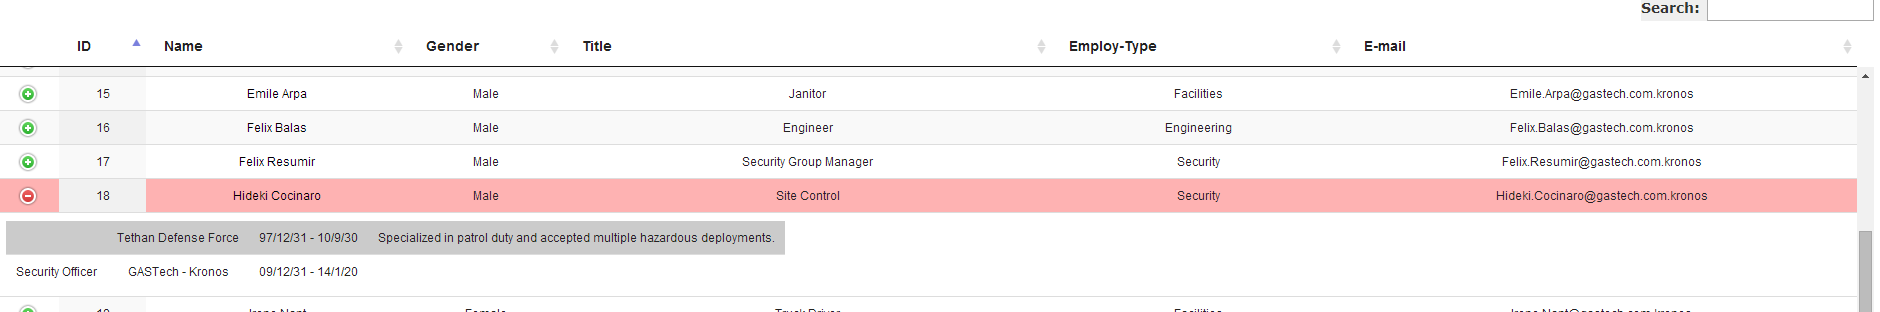
\includegraphics[width=3in]{SingleExperienceLine2.png}
  \caption{Identify conflicts and check it using detailed description}
\end{figure}

\subsection{News timeline}
News timeline is designed to provide a quick view for the user to grab the development of an event and then select a focus point to analysis. 
\par
As the volume of news data is large, simply display news in a timing can be imbalance and with a lot of overlapping in a period of time. Semantic zooming is used in News Timeline, which make it possible to provide a compact view in the timeline when the time range is long and provide news position precisely when the range is short.
\par
Aside rooming function, News Timeline provide visual set operation on timelines. Every time user search a keyword, a new timeline will be generated and display on the screen. As timeline operation are allowed for user, a user can do set operations between them to refine the result he find. Draggable dialogs are also provided to refine data, user can pick up important news he find and arrange them in the timeline by dragging to prepare for further investigation.
\begin{figure}[htb!]
  \centering
  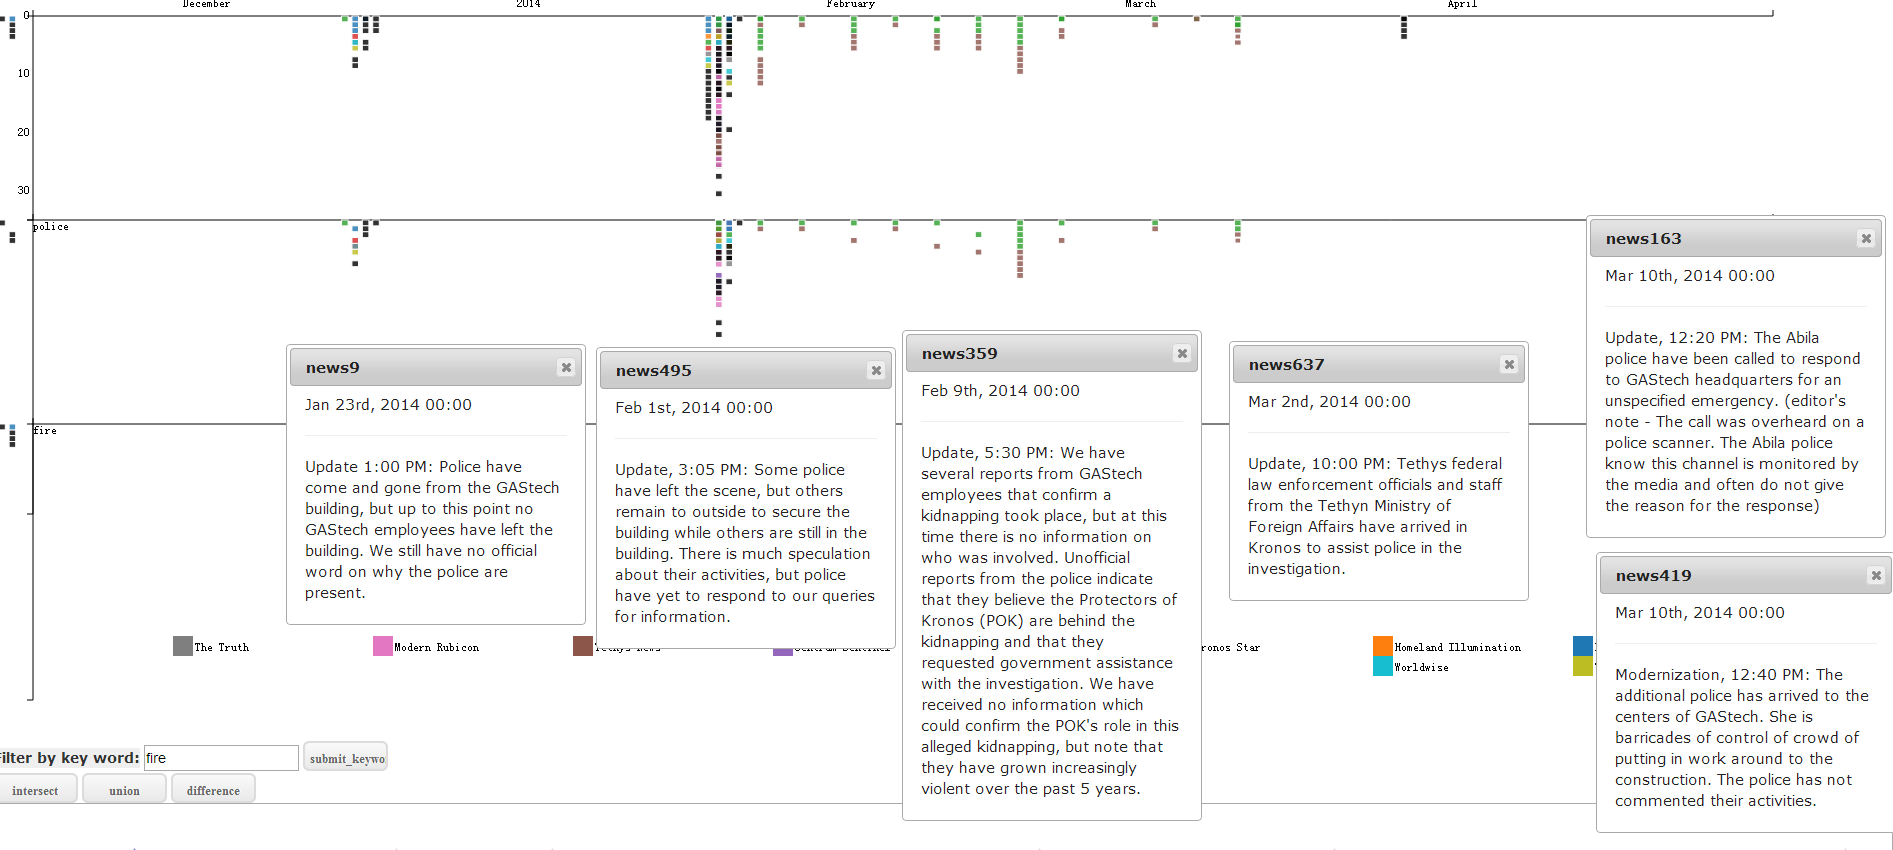
\includegraphics[width=3in]{image017.png}
  \caption{Operational NewsTimeline}
\end{figure}

\subsection{Email Reader}
\todo{Is that complete?}
\subsubsection{Design And Overview}
In MC1 we have email headers from two weeks of internal GAStech company email, we can get a social network from this data and then discover communities. For MC1, we need to reveal the connections between GAStech employees and to find suspectable clues including the subject of emails. If there is an email containing words related to POK, then we can try to find the connections between the sender of the email's community and POK. Therefore we implemented a visual analytic tool for email headers based on D3.js. The tool is easy to use and effective to discover communities. 

\subsubsection{Layout And User Interactions}
Our tool's layout containing four components, filters, email sending and receiving timeline, email headers view, and community view.
After selecting an employee through the filter, his/her email records will be depicted on the timeline, the contents of email headers will be put in the email headers view and some communities including him/her will be showed in the community view.  \\
Users can interact with the layout both directly and indirectly, including selecting employees, filtering by keywords and limiting. 
\begin{figure}[htb]
  \centering
  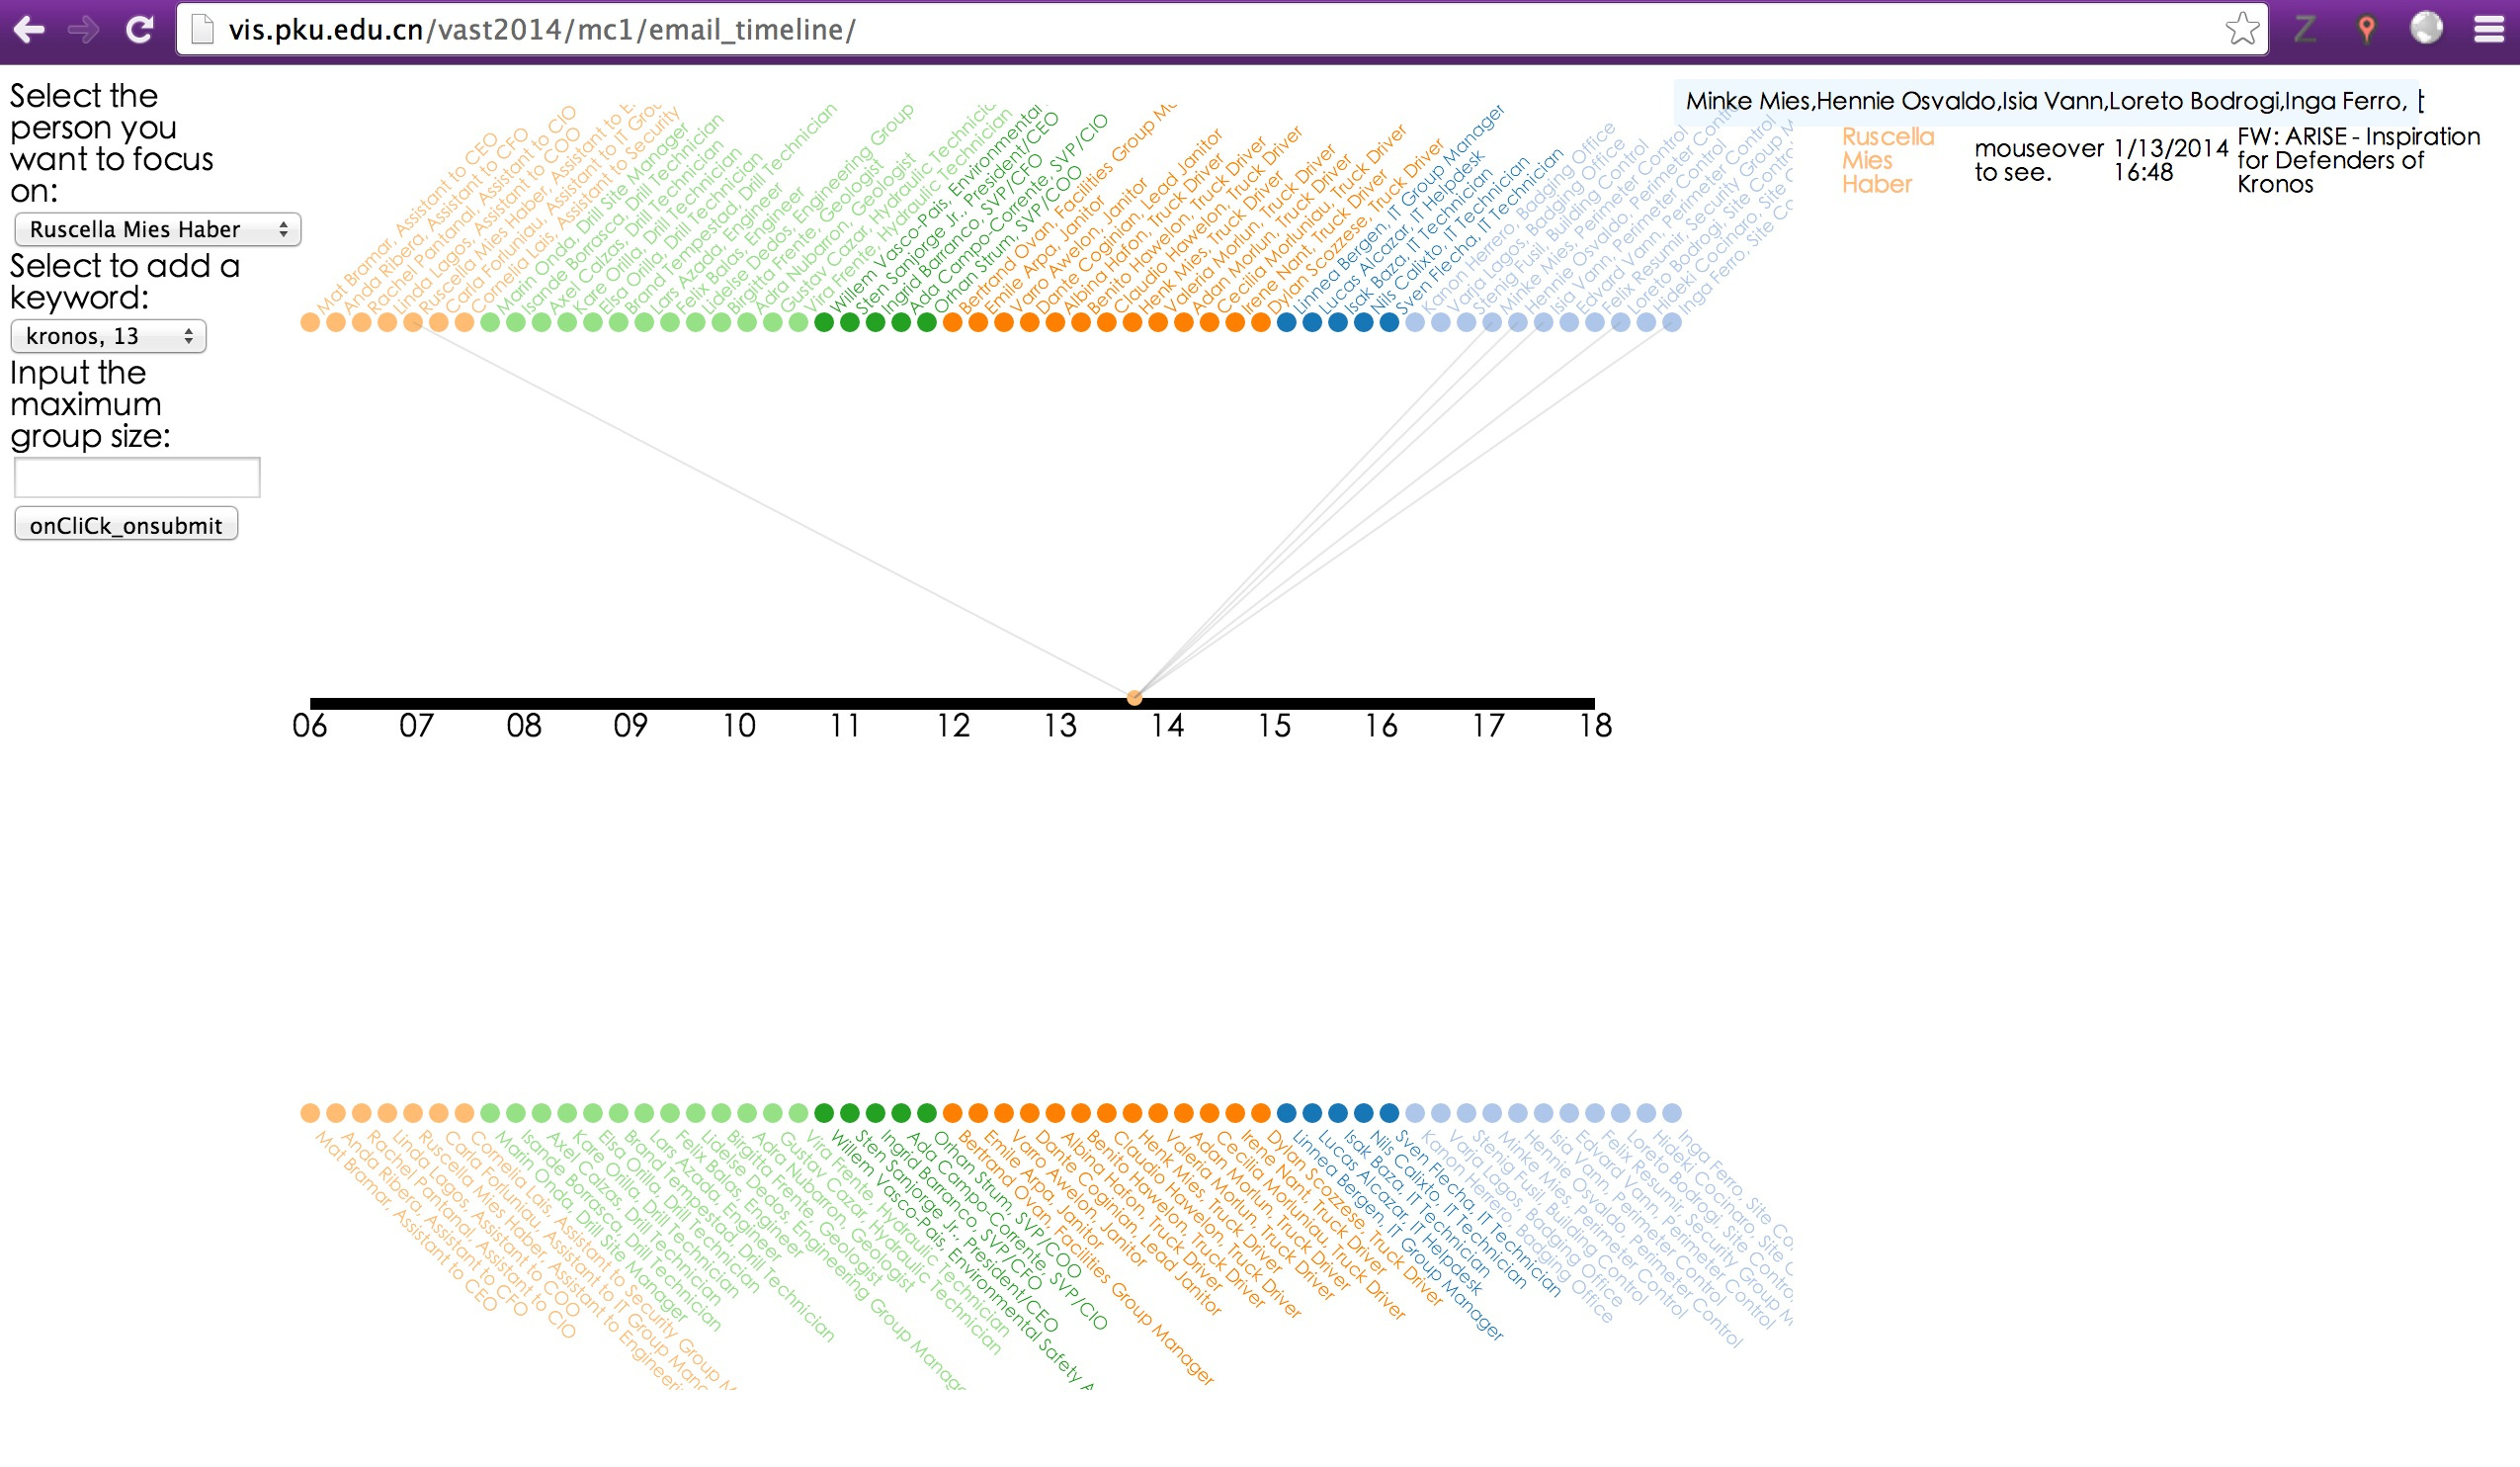
\includegraphics[width=3in]{image_et.png}
  \caption{Email Reader}
\end{figure}

\section{Data Exploration}
In this section, we introduce how we use \projectname\ along with analysis tools like Jigsaw, Gephi to analysis MC1 data.
\par
As our tool only provides an overview of the whole data, we still need to use Jigsaw to assist the analysis process. And general analysis includes following steps:
1. Read report on POK and GAStech to identify important people involved in the conflicts.
2. With important entities identified, using News Timeline to refine keywords.
3. Cooperated with Jigsaw to read news articles and find relationship between POK and GAStech.
4. Identify important groups and identify suspicious people with Resume Reader and Email Reader.
5. Go on for another round of exploration.
6. Present our find with the help of Gephi.
\par
And with rounds of explaration, we can finally get enough information to answer questions.

\section{Conclusion}
\projectname\ provide the user the ability to grab important events from huge volume of news ariticles and the ability to analysis conflict data of employee resume. And with the help of \projectname, we successfully find out a group of GAStech people are suspicious to the kidnap event. \todo{Add more conclusion.}

%% if specified like this the section will be ommitted in review mode
\acknowledgements{
We have special thanks to Miss Dong Liu for her dedicated exploration with raw materials to inspire our design on visualization tools.
}

\bibliographystyle{abbrv}
%%use following if all content of bibtex file should be shown
%\nocite{*}
\bibliography{template}
\end{document}
